\documentclass{article}

% Language setting
% Replace `english' with e.g. `spanish' to change the document language
\usepackage[english]{babel}

% Set page size and margins
% Replace `letterpaper' with `a4paper' for UK/EU standard size
\usepackage[letterpaper,top=1.5cm,bottom=1.5cm,left=1.25cm,right=1.25cm,marginparwidth=1.75cm]{geometry}

% Useful packages
\usepackage{amsmath}
\usepackage{graphicx}
\usepackage{subcaption} % For subfigures
\usepackage[colorlinks=true, allcolors=blue]{hyperref}
\usepackage{float}

\title{Machine Learning Exercise 0}
\author{Amélie Assmayr (12007770) \and
        Konstantinos Damanakis (12106343) \and
        Teresa Schuch (12007762)}

\begin{document}
\maketitle

\section{Introduction}

In this Exercise we have chosen two datasets: Laptop Prices and Road Traffic Accidents. The Laptop Prices dataset will be utilized to develop models for predicting laptop prices based on various specifications, while the Road Traffic Accidents dataset will be employed to classify the severity of accidents in the capital city of Ethiopia. 
\par We decided on those two datasets because they enable us to try various and diverse techniques within our framework as they cover different aspects. The Laptop Prices dataset is clean, with no missing values, and consists of 15 features. On the other hand, the Road Traffic Accidents dataset contains 20.057 missing values in 16 variables and includes over 30 features, making the pre-processing steps for this dataset more important and complex.

\section{Dataset 1: Laptop Prices}

The Laptop Price dataset contains information about various laptops and their prices in Euros. It includes detailed specifications that describe each laptop's features and capabilities. With this, we aim to build a machine learning model that can predict laptop prices based on these specifications. 
\par The motivation of choosing the Laptop Price dataset is its importance in real-life situations, since most people today rely on laptops for work, education and entertainment. Understanding the price trends can help consumers make informed purchasing decisions, making this dataset highly relevant in today’s technology-driven world. Additionally, the variety of features in the dataset, including both categorical and numeric data makes it ideal for experimenting with feature engineering and different machine learning methods.

\subsection{Attribute Types}

The dataset has 2275 instances and 15 variables. Among these variables, there are 8 nominal, 2 ordinal and 5 metrics. The variables together with their datatypes can be seen in the table below:

\begin{table}[H]
    \small
    \parbox{.40\linewidth}{
        \begin{tabular}{l|r}
            \textbf{Variable} & \textbf{Datatype} \\\hline
            Company & nominal \\
            Product & nominal \\
            Type Name & nominal \\
            Inches & ratio quantity \\
            Screen Resolution & ordinal \\
            CPU Company & nominal \\
            CPU Type & nominal \\
            CPU Frequency (GHz) & ratio quantity
        \end{tabular}
}
    \hfill
    \parbox{.40\linewidth}{
        \begin{tabular}{l|r}
            \textbf{Variable} & \textbf{Datatype} \\\hline
            RAM (GB) & ratio quantity \\
            Memory & ordinal \\
            GPU Company & nominal \\
            GPU Type & nominal \\
            Operating System & nominal \\
            Weight (kg) & ratio quantity \\
            Price (Euro) & ratio quantity 
        \end{tabular}}
        
\end{table}
The histograms of two attributes are given below as an example, where Fig~\ref{fig:figure1} shows the distribution of the RAM (numeric attribute) and Fig~\ref{fig:figure2} shows the distribution of the CPU type (categorical attribute) \footnote{Due to limited space, only a selected number of variables were displayed visually for both datasets. All additional plots generated can be viewed
\href{https://github.com/amyteresakostas/MachineLearning_2024_TUW/tree/main/ML_Exercise0}{here}}. Given that the CPU Type has many distinct values, only the top 10 values are presented to maintain clarity in visualization.

 \begin{figure}[H]
    \centering 
    \begin{subfigure}[b]{0.35\textwidth}
        \centering
        \includegraphics[width=\linewidth]{Barplot_RAM.jpeg} 
        \caption{Histogram RAM}
        \label{fig:figure1}
    \end{subfigure}
     \hspace{0.05\textwidth} % Adjust space between figures
    \begin{subfigure}[b]{0.35\textwidth}
        \centering
        \includegraphics[width=\linewidth]{Barplot_CPUTypes.png} 
        \caption{Barplot CPU Types}
        \label{fig:figure2}
    \end{subfigure}
    \caption{Examples of attributes for laptop price dataset}
    \label{fig:two_figures}
\end{figure}

\subsection{Target attribute}
The target variable is the laptop price. Estimating this variable through regression analysis can provide retailers with crucial insights into expected revenues before official pricing is announced. The histogram below illustrates the distribution of laptop prices, revealing that most laptops are priced between 400 and 800 €. However, the mean price stands at 1135 €, with a median of 989 €. Calculating the median makes sense since we can see that there a a few laptops that cost between 5000 and 6000 € which is much higher than the rest. Still these outliers are valid values. The prices range between 174€ and 6099€.

\begin{figure}[H]
\centering
\includegraphics[width=0.3\linewidth]{Histogram_Price.png}
\caption{\label{fig:hist:price}Histogramm Laptop Price}
\end{figure}

\section{Dataset 2: Road Traffic Accidents}

The Road Traffic Accidents dataset includes instances of road traffic accidents recorded in the years between 2017 and 2020 in Addis Ababa, capital city of Ethiopia. This dataset contains information regarding the number and characteristics of the vehicles and the drivers that took part in the accidents, the conditions and the casualties that happened as a result of these unfortunate events.
\par We chose this dataset because it addresses a critical public safety issue that affects many people. A study of this data and a development of a machine learning model would enable the classification and prediction of the severity of the accident based on the different features that lead to or are involved in the accident. This analysis can help identify the major causes and factors contributing to road safety, which is essential for improving transportation policies and reducing accidents. 

\subsection{Attribute Types}

The data contains 31 attributes related to the accident and the target variable which is the severity of the accident. There are 12316 samples/cases recorded while missing data can be observed in 16 features. Among the features, there 24 nominal, 1 ordinal and 7 metric variables. Preprocessing steps are necessary to handle the missing values. In the following table all 31 attributes are presented together with their type of data and number of missing values:

\begin{table}[H]
    \small
    \parbox{.45\linewidth}{
        \begin{tabular}{c|c|c|c}
            \textbf{Variable} & \textbf{Datatype} &
            \textbf{Unique} &  \textbf{Missing}\\\hline
            Time & ratio & / & - \\
            Day of Week & nominal & 7 & -\\
            Age of Driver & ratio & / & -\\
            Sex of Driver & nominal & 3& -\\
            Educational Level & nominal &7 &741\\
            Vehicle-Driver Relation & nominal & 4 & 579 \\
            Driving Experience & ratio  & / & 829\\
            Vehicle Type & nominal & 17 & 950\\
            Vehicle Owner & nominal & 4 & 482\\
            Vehicle Service Year & ratio & / & 3.928\\
            Defect of Vehicle & nominal & 3 & 4.427\\
            Accident Area & nominal & 14 & 239\\
            Lanes or Medians & nominal & 7 & 385\\
            Road Alignment & nominal & 9& 142\\
            Junction Type & nominal & 8 & 887\\
            Road Surface Type & nominal  & 4 &172
        \end{tabular}
}
    \hfill
    \parbox{.45\linewidth}{
        \begin{tabular}{c|c|c|c}
            \textbf{Variable} & \textbf{Datatype} &
            \textbf{Unique} & \textbf{Missing} \\\hline
            Road Surface Condition & nominal & 4 & -\\
            Light Condition & nominal & 4 & -\\
            Weather Condition & nominal & 9 & -\\
            Collision Type & nominal & 10 & 155\\
            Number of Vehicles & ratio & / & -\\
            Number of Casualty & ratio & / & -\\
            Vehicle Movement & nominal & 13 & 308\\
            Casualty Class & nominal & 4 & -\\
            Sex of Casualty & nominal & 3 & -\\
            Age of Casualty & ratio & / & -\\
            Casualty Severity & ordinal & 4 & -\\
            Work of Casualty & nominal & 7 & 3.198\\
            Fitness of Casualty & nominal & 5 & 2.635\\
            Pedestrian Movement & nominal & 9 & -\\
            Cause of Accident & nominal & 20 & -\\
            Severity of Accident & nominal & 3 & -
        \end{tabular}}
\end{table}
It should be noted that most of the numeric variables in the dataset are grouped into intervals. For example, the driving experience, although it could be considered ordinal type, it is given in intervals of years (e.g 2-5 years) converting it into a ratio variable. In Figure \ref{fig:two_figures2}, two histograms of selected attributes are shown, namely the time of the accident and the type of collisions:

\begin{figure}[H]
    \centering
    \begin{subfigure}[b]{0.4\textwidth}
        \centering
        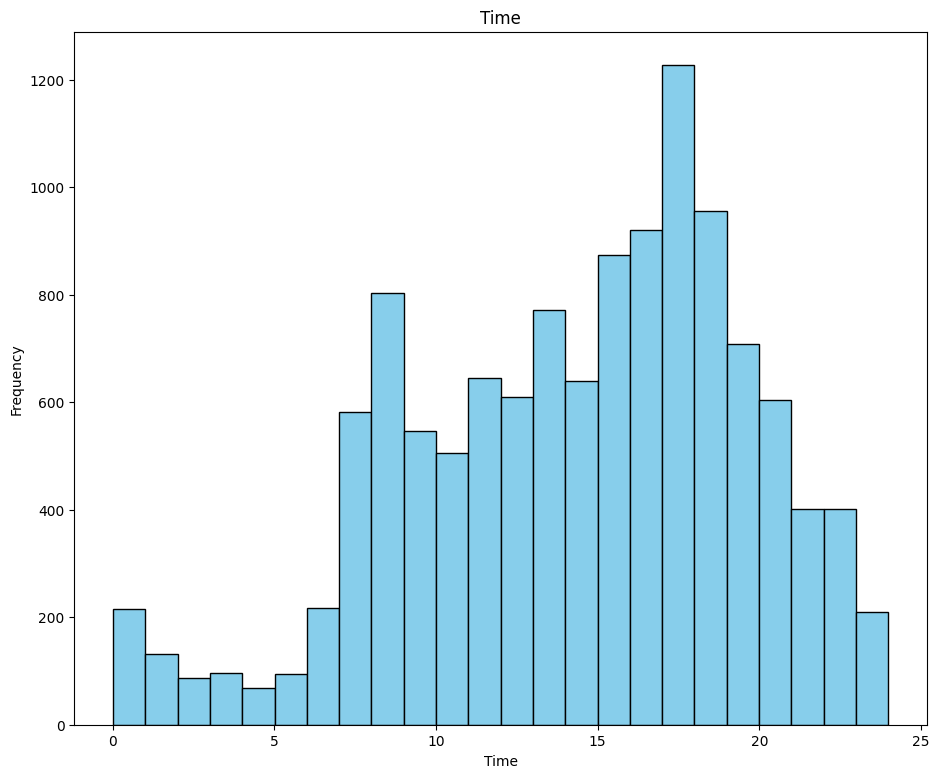
\includegraphics[width=\linewidth]{Time.png} 
        \caption{Time}
        \label{fig:figure11}
    \end{subfigure}
    \hspace{0.05\textwidth}
    \begin{subfigure}[b]{0.4\textwidth}
        \centering
        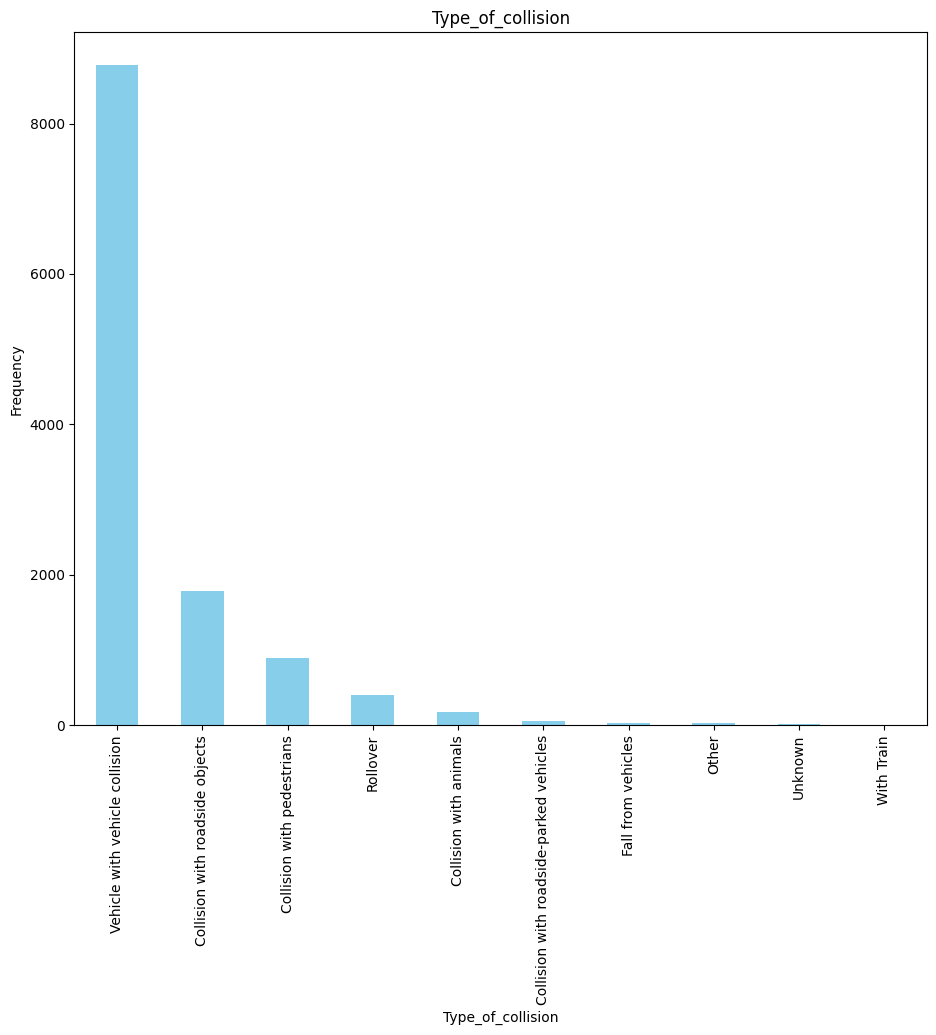
\includegraphics[width=\linewidth]{Type_of_collision.png} 
        \caption{Barplot Type of Collisions}
        \label{fig:figure22}
    \end{subfigure}
    \caption{Examples of attributes for road accidents dataset}
    \label{fig:two_figures2}
\end{figure}
\subsection{Target Attribute}

The target variable is the severity of the accident. It is classified into the three following classes: Light, Serious and Fatal Injury. While the severity could be considered an ordinal variable, we will treat it as nominal, framing the task as a multi-class classification problem. Figure~\ref{fig:hist:price} shows the distribution of these classes. It can be seen that the classes are really unevenly distributed. Most accidents fall under the "Slight Injury" category, with 10,415 instances, followed by "Serious Injury" with 1,743 instances, and only 158 accidents classified as "Fatal Injury." This imbalance is a critical factor to consider when developing and evaluating the model.

\begin{figure}[H]
\centering
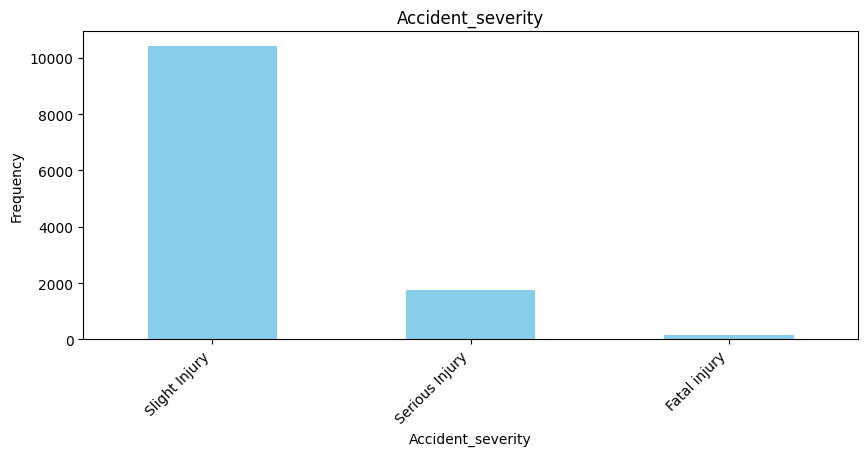
\includegraphics[width=0.4\linewidth]{Accident_severity.png}
\caption{\label{fig:hist:price}Barplot Accident Severity}
\end{figure}


\end{document}